\section{Introduction}
\dropcap{B}rain Machine Interfaces (BMI) \citep{liu2024cognitive} facilitate the translation of neural activity into actionable commands, enabling individuals to control external devices and systems through their thoughts and attention~\citep{coyle2007brain,lee2017brain}. Compared to traditional bulky EEG setups~\citep{van2012brain}, one of the emerging avenues towards practical and wearable \glspl{EEG} devices are systems based on motor imagery signals due to their intuitiveness and no external dependency on (e.g., visual) stimuli. These have been use in stroke rehabilitation \citep{khan2020review}. Several works in literature have considered using this technology to control robot manipulators~\citep{schiatti2017soft,aldini2019effect,lee2024noir}. % more citations: bhattacharyya2017motor, liu2018motor

However, the state-of-the-art classifiers on few-channel, online \gls{EEG} signals are still limited in achieving an accuracy of 65-75 \si{\percent}~\citep{arpaia2022non, lee2024noir} and are prone to producing outliers, which make it very challenging to operate robots safely and robustly using these techniques~\citep{liu2024cognitive}. In (rigid) robotics literature, this has been addressed by relying on force-based (i.e., impedance) control~\citep{schiatti2017soft} and by making the robot's behavior more predictable~\citep{aldini2019effect}.
%
%from a perspective of real-life scenarios along with several factors taken into consideration, such as a limited number of channels, operating an interface}~\textcolor{orange}{},
% Additionally, various factors such as the human brain being uncertain at times, low ITR rate,and low discrimination capacity of the human brain can inevitably lead to unintended movements and therefore pose a potential safety hazard to both humans and objects close to the robot.\textcolor{red}{!!!!{/cite}}
%
In this chapter, we follow a different path and investigate \textit{embodying} safety by pairing soft robots~\citep{rus2015design, della2020softencyclopedia} 
with \gls{BMI}. This way, risks can be mitigated, and more natural interactions with an unstructured environment can be achieved by relying on structural compliance.

\begin{figure}[hbt]
    \centering
    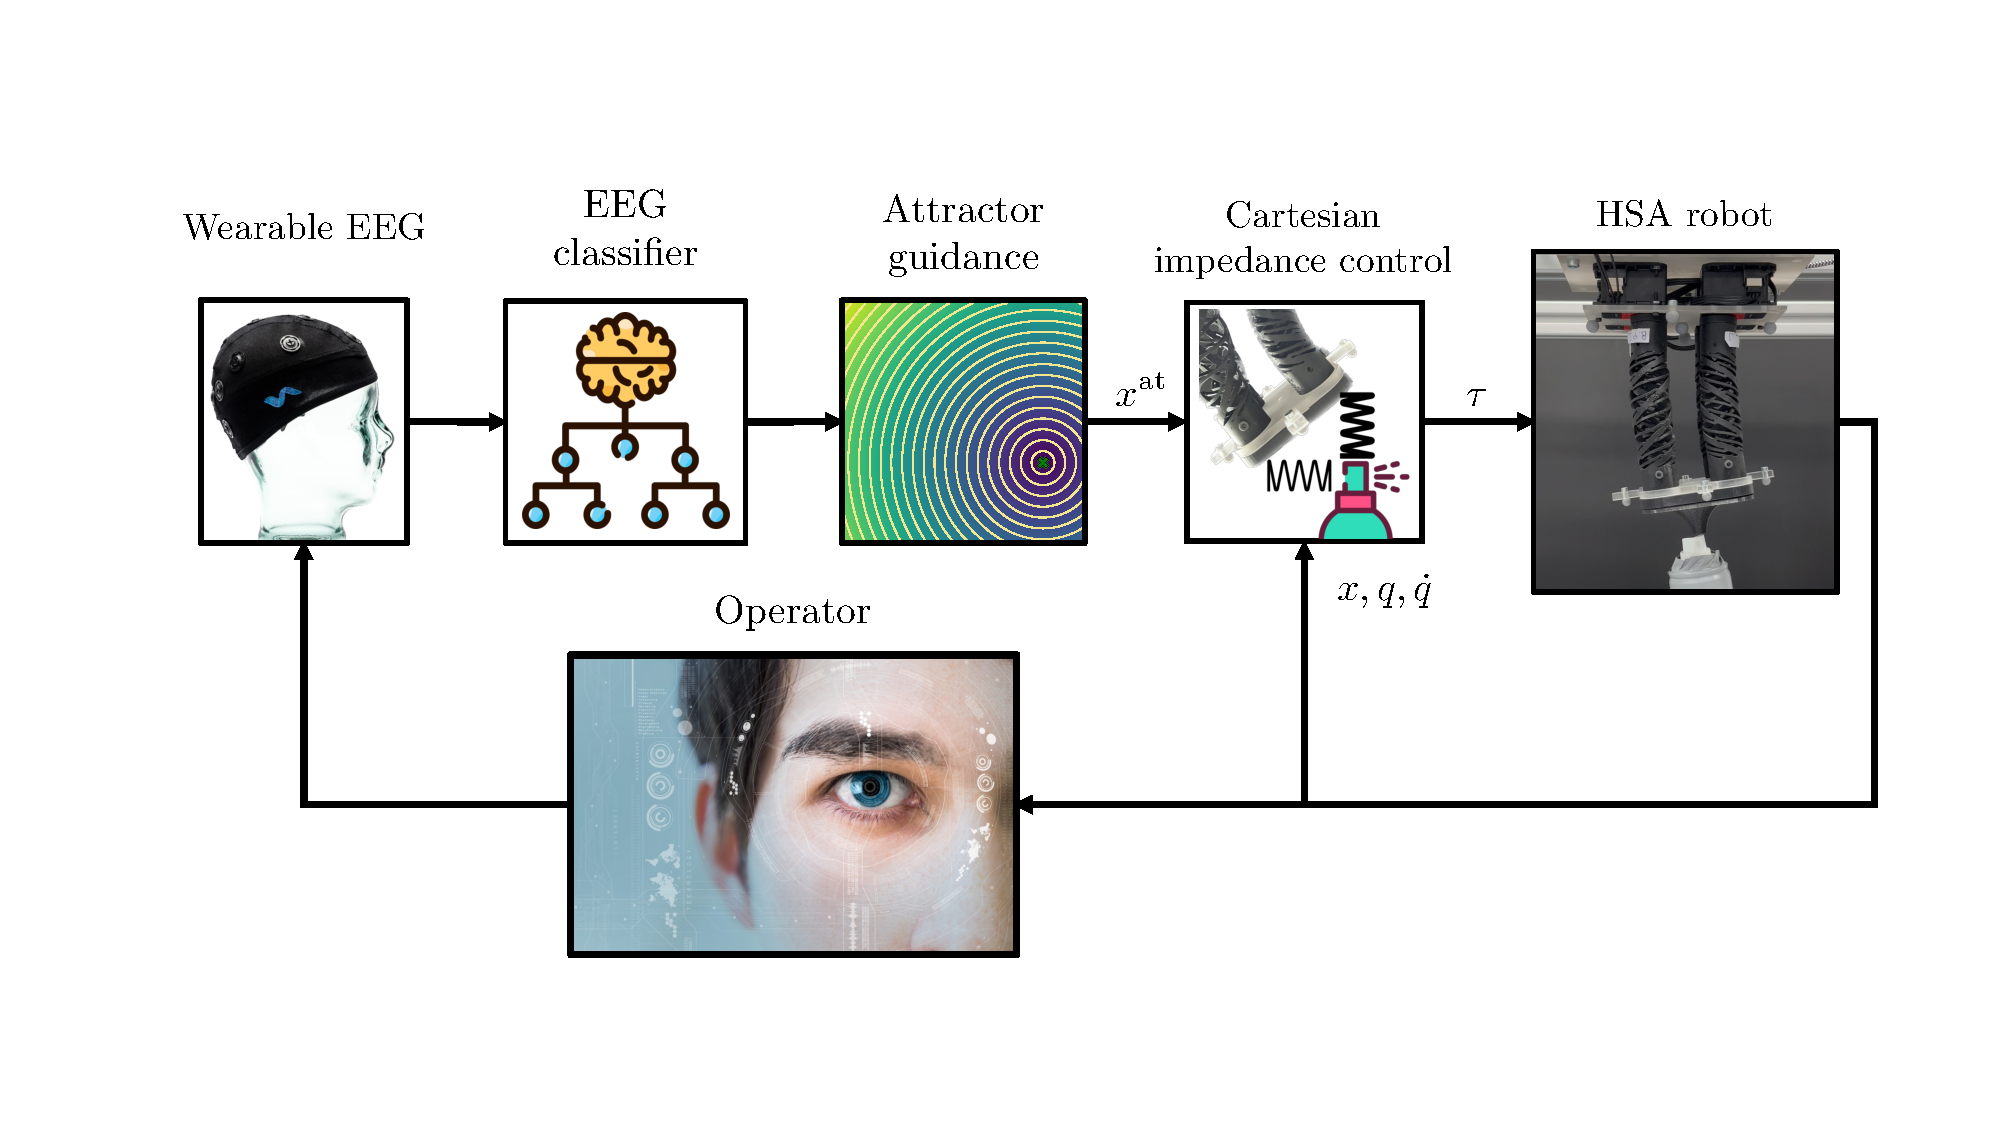
\includegraphics[width=0.7\columnwidth]{braincontrol/figures/control_scheme/control_scheme_high_level_overview_cropped.pdf}
    \caption{High-level control scheme of an operator steering an \gls{HSA} robot with brain signals. We leverage the \gls{EEG} signal classifications for guiding an attractor in the plane. Subsequently, an impedance controller is designed to shape the impedance in Cartesian space and render the attractor to be a globally asymptotically stable equilibrium of the potential.}
    \label{fig:braincontrol:control_scheme_high_level_overview}
\end{figure}

While \gls{BMI}-based assistance has been investigated with a focus on 
% exoskeletons~\citep{wairagkar2016movement, araujo2021development} 
soft exosuits assisting hand-rehabilitation ~\citep{zhang2019eeg} or with strenuous arm acitivites~\citep{tacca2022neuro}, 
% \textcolor{red}{TODO: insert combination of a) soft robotics and BCI are both emerging fields, b) most of the focus has been on binary decisions }
it is still an open challenge how \gls{BMI} can be used for controlling soft manipulators. 
%One key reason for existing strategies developed for soft exosuits and hands not being directly applicable to more complex soft robots is that those strategies restricted the interface to binary decisions such as \emph{open} / \emph{close}. To overcome these limitations, 
In this chapter, we make a first step towards solving this challenge by proposing a pipeline (see Fig. \ref{fig:braincontrol:control_scheme_high_level_overview}) that lets the user steer the soft robot's end-effector in Cartesian space. The two key ingredients are a novel mapping strategy transforming the brain signals into meaningful references and Cartesian impedance control. The latter is essential because it allows for preserving the robot's compliance in closed-loop \citep{della2017controlling}. We build the proposed \gls{BMI} pipeline around a \gls{HSA} soft robot \citep{stolzle2023modelling, stolzle2024experimental}, % truby2021recipe
which relies on architected metamaterials and electrical actuation to elongate, bend, and twist.
\gls{HSA} robots are an excellent match for our test case of assisting with \gls{ADL}, as they can be portable because of their electrical actuation, they are compact and combine many \glspl{DOF} in one segment, and easy to manufacture via 3D printing~\citep{truby2021recipe}.
% This makes the control problem especially challenging because of the peculiarity of these systems' dynamics, namely underactuation and non-affinity in control. % We provide more details on innovation from the model-based control standpoint in Section~\ref{sub:braincontrol:computational_controller}.

\begin{figure}[hbt]
    \centering
    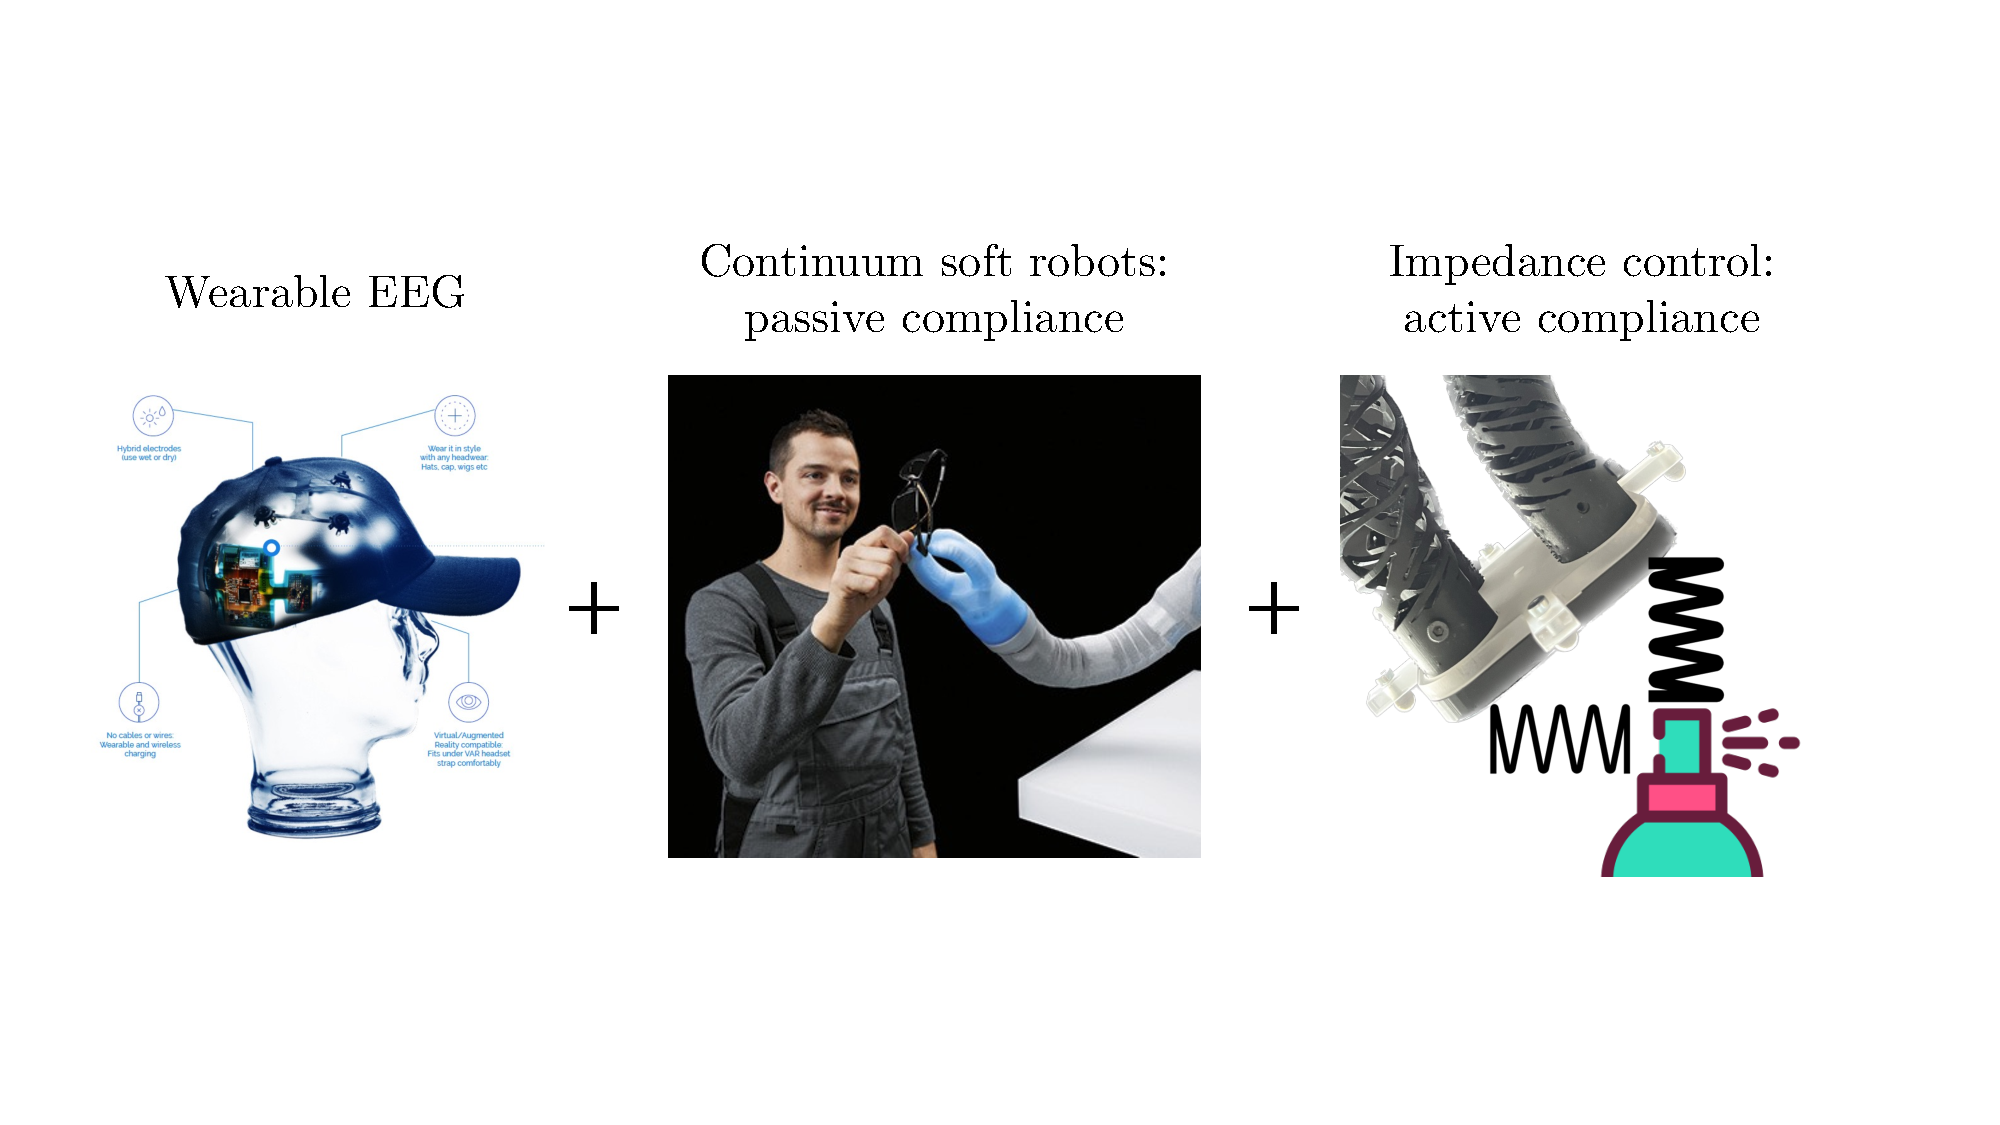
\includegraphics[width=0.7\textwidth]{braincontrol/figures/embodied_computational_intelligence/embodied_and_computational_intelligence_cropped.pdf}
    \caption{In this work we propose combining wearable \gls{EEG} devices with continuum soft robots and impedance control. The classification accuracy of motor imagery based on signals from few-channel, wearable \gls{EEG} devices is currently limited to less than \SI{75}{\percent}. The inevitable operation errors can be accepted by establishing both passive and active compliance: The embodied intelligence of soft robots guarantees safety during interactions with the environment, which is complemented by an impedance controller that allows us to design the Cartesian stiffness and damping characteristics of the robot.}
    \label{fig:braincontrol:embodied_computational_intelligence}
\end{figure}
 
We quantitatively verify the entire approach on mind-controlled setpoint regulation involving tracking a reference consisting of nine-step functions and demonstrate the qualitative behavior when assisting with a simple daily living activity. 
% Furthermore, we compare the performance of our motor imagery-based control to approaches giving the computational controller access to the privileged information of setpoints, which can considered to be an upper bound on performance.
Furthermore, we compare the performance of our motor imagery-based control to an approach that can be considered an upper bound on performance: The control using keyboard inputs is a very effective and efficient \gls{HMI} strategy but requires the user to always interact physically with a keyboard,
which is not always desirable or possible (e.g., for users with disabilities).
% and (b) giving the computational controller access to the privileged information of setpoints.
% This control strategy now allows us to define the stiffness of the closed-loop system in Cartesian space. We verify the controller on the task of pressing the button of a perfume, which requires high stiffness in the normal direction of the interaction and flexibility in the tangential direction, allowing the soft robots to adapt to the environment interaction with physical intelligence.

Our contribution is establishing a \gls{BMI} strategy for continuum soft robots. This strategy is supported by experiments in which we perform setpoint regulation with a planar \gls{HSA} robot and motor imagery, which we experimentally validated on a simple \gls{ADL} task involving environment interaction: the user needs to steer the end-effector towards the tip of a hairspray container, apply force for releasing the fluid, and finally let the robot retreat from the contact.          

A video attachment to this chapter, including recordings of experimental results, can be found on YouTube\footnote{\url{https://youtu.be/wZTOxBPZmPc}}.
Furthermore, we have open-sourced our code, including the OpenVibe pipeline, on GitHub\footnote{\url{https://github.com/tud-phi/sr-brain-control}}.